% Options for packages loaded elsewhere
\PassOptionsToPackage{unicode}{hyperref}
\PassOptionsToPackage{hyphens}{url}
\PassOptionsToPackage{dvipsnames,svgnames,x11names}{xcolor}
%
\documentclass[
  11pt,
  ignorenonframetext,
]{beamer}
\usepackage{pgfpages}
\setbeamertemplate{caption}[numbered]
\setbeamertemplate{caption label separator}{: }
\setbeamercolor{caption name}{fg=normal text.fg}
\beamertemplatenavigationsymbolsempty
% Prevent slide breaks in the middle of a paragraph
\widowpenalties 1 10000
\raggedbottom
\setbeamertemplate{part page}{
  \centering
  \begin{beamercolorbox}[sep=16pt,center]{part title}
    \usebeamerfont{part title}\insertpart\par
  \end{beamercolorbox}
}
\setbeamertemplate{section page}{
  \centering
  \begin{beamercolorbox}[sep=12pt,center]{part title}
    \usebeamerfont{section title}\insertsection\par
  \end{beamercolorbox}
}
\setbeamertemplate{subsection page}{
  \centering
  \begin{beamercolorbox}[sep=8pt,center]{part title}
    \usebeamerfont{subsection title}\insertsubsection\par
  \end{beamercolorbox}
}
\AtBeginPart{
  \frame{\partpage}
}
\AtBeginSection{
  \ifbibliography
  \else
    \frame{\sectionpage}
  \fi
}
\AtBeginSubsection{
  \frame{\subsectionpage}
}

\usepackage{amsmath,amssymb}
\usepackage{lmodern}
\usepackage{iftex}
\ifPDFTeX
  \usepackage[T1]{fontenc}
  \usepackage[utf8]{inputenc}
  \usepackage{textcomp} % provide euro and other symbols
\else % if luatex or xetex
  \usepackage{unicode-math}
  \defaultfontfeatures{Scale=MatchLowercase}
  \defaultfontfeatures[\rmfamily]{Ligatures=TeX,Scale=1}
\fi
% Use upquote if available, for straight quotes in verbatim environments
\IfFileExists{upquote.sty}{\usepackage{upquote}}{}
\IfFileExists{microtype.sty}{% use microtype if available
  \usepackage[]{microtype}
  \UseMicrotypeSet[protrusion]{basicmath} % disable protrusion for tt fonts
}{}
\makeatletter
\@ifundefined{KOMAClassName}{% if non-KOMA class
  \IfFileExists{parskip.sty}{%
    \usepackage{parskip}
  }{% else
    \setlength{\parindent}{0pt}
    \setlength{\parskip}{6pt plus 2pt minus 1pt}}
}{% if KOMA class
  \KOMAoptions{parskip=half}}
\makeatother
\usepackage{xcolor}
\newif\ifbibliography
\setlength{\emergencystretch}{3em} % prevent overfull lines
\setcounter{secnumdepth}{-\maxdimen} % remove section numbering


\providecommand{\tightlist}{%
  \setlength{\itemsep}{0pt}\setlength{\parskip}{0pt}}\usepackage{longtable,booktabs,array}
\usepackage{calc} % for calculating minipage widths
\usepackage{caption}
% Make caption package work with longtable
\makeatletter
\def\fnum@table{\tablename~\thetable}
\makeatother
\usepackage{graphicx}
\makeatletter
\def\maxwidth{\ifdim\Gin@nat@width>\linewidth\linewidth\else\Gin@nat@width\fi}
\def\maxheight{\ifdim\Gin@nat@height>\textheight\textheight\else\Gin@nat@height\fi}
\makeatother
% Scale images if necessary, so that they will not overflow the page
% margins by default, and it is still possible to overwrite the defaults
% using explicit options in \includegraphics[width, height, ...]{}
\setkeys{Gin}{width=\maxwidth,height=\maxheight,keepaspectratio}
% Set default figure placement to htbp
\makeatletter
\def\fps@figure{htbp}
\makeatother
\newlength{\cslhangindent}
\setlength{\cslhangindent}{1.5em}
\newlength{\csllabelwidth}
\setlength{\csllabelwidth}{3em}
\newlength{\cslentryspacingunit} % times entry-spacing
\setlength{\cslentryspacingunit}{\parskip}
\newenvironment{CSLReferences}[2] % #1 hanging-ident, #2 entry spacing
 {% don't indent paragraphs
  \setlength{\parindent}{0pt}
  % turn on hanging indent if param 1 is 1
  \ifodd #1
  \let\oldpar\par
  \def\par{\hangindent=\cslhangindent\oldpar}
  \fi
  % set entry spacing
  \setlength{\parskip}{#2\cslentryspacingunit}
 }%
 {}
\usepackage{calc}
\newcommand{\CSLBlock}[1]{#1\hfill\break}
\newcommand{\CSLLeftMargin}[1]{\parbox[t]{\csllabelwidth}{#1}}
\newcommand{\CSLRightInline}[1]{\parbox[t]{\linewidth - \csllabelwidth}{#1}\break}
\newcommand{\CSLIndent}[1]{\hspace{\cslhangindent}#1}

\setbeamertemplate{itemize items}{\raisebox{0.15\height}{$\vcenter{\hbox{\scalebox{0.5}{\usebeamercolor[fg]{structure} $\blacktriangleright$}}}$}}
\usepackage{setspace}\setstretch{1.15}
\usepackage{etoolbox} \newcommand{\zerodisplayskips}{ \setlength{\abovedisplayskip}{0.25\baselineskip} \setlength{\belowdisplayskip}{0.25\baselineskip} \setlength{\abovedisplayshortskip}{0.15\baselineskip} \setlength{\belowdisplayshortskip}{0.15\baselineskip}} \appto{\normalsize}{\zerodisplayskips} \appto{\small}{\zerodisplayskips} \appto{\footnotesize}{\zerodisplayskips}
\setlength{\leftmargini}{4pt}
\setlength{\leftmarginii}{12pt}
\setbeamertemplate{itemize/enumerate body begin}{\normalsize}
\setbeamertemplate{itemize/enumerate subbody begin}{\normalsize}
\ifdefined\Shaded\renewenvironment{Shaded}{\small\begin{tcolorbox}[top=2pt, bottom=0pt, borderline west={3pt}{0pt}{shadecolor}, interior hidden, frame hidden, enhanced, boxrule=0pt, sharp corners, breakable]}{\end{tcolorbox}}\fi
\usepackage{verbatim}
\makeatletter \patchcmd{\@verbatim}{\verbatim@font}{\small\verbatim@font}{}{} \makeatother
\usepackage{pgf}
\usepackage{tikz}
\usetikzlibrary{graphs, arrows, automata, shadings}
\tikzset{invisible/.style={opacity=0}, visible on/.style={alt={#1{}{invisible}}}, alt/.code args={<#1>#2#3}{\alt<#1>{\pgfkeysalso{#2}}{\pgfkeysalso{#3}}}}
\usepackage{adjustbox}
\makeatletter
\makeatother
\makeatletter
\makeatother
\makeatletter
\@ifpackageloaded{caption}{}{\usepackage{caption}}
\AtBeginDocument{%
\ifdefined\contentsname
  \renewcommand*\contentsname{Table of contents}
\else
  \newcommand\contentsname{Table of contents}
\fi
\ifdefined\listfigurename
  \renewcommand*\listfigurename{List of Figures}
\else
  \newcommand\listfigurename{List of Figures}
\fi
\ifdefined\listtablename
  \renewcommand*\listtablename{List of Tables}
\else
  \newcommand\listtablename{List of Tables}
\fi
\ifdefined\figurename
  \renewcommand*\figurename{Figure}
\else
  \newcommand\figurename{Figure}
\fi
\ifdefined\tablename
  \renewcommand*\tablename{Table}
\else
  \newcommand\tablename{Table}
\fi
}
\@ifpackageloaded{float}{}{\usepackage{float}}
\floatstyle{ruled}
\@ifundefined{c@chapter}{\newfloat{codelisting}{h}{lop}}{\newfloat{codelisting}{h}{lop}[chapter]}
\floatname{codelisting}{Listing}
\newcommand*\listoflistings{\listof{codelisting}{List of Listings}}
\makeatother
\makeatletter
\@ifpackageloaded{caption}{}{\usepackage{caption}}
\@ifpackageloaded{subcaption}{}{\usepackage{subcaption}}
\makeatother
\makeatletter
\@ifpackageloaded{tcolorbox}{}{\usepackage[many]{tcolorbox}}
\makeatother
\makeatletter
\@ifundefined{shadecolor}{\definecolor{shadecolor}{rgb}{.97, .97, .97}}
\makeatother
\makeatletter
\makeatother
\ifLuaTeX
  \usepackage{selnolig}  % disable illegal ligatures
\fi
\IfFileExists{bookmark.sty}{\usepackage{bookmark}}{\usepackage{hyperref}}
\IfFileExists{xurl.sty}{\usepackage{xurl}}{} % add URL line breaks if available
\urlstyle{same} % disable monospaced font for URLs
\hypersetup{
  pdftitle={Modeling COVID-19 Incidence},
  colorlinks=true,
  linkcolor={Maroon},
  filecolor={Maroon},
  citecolor={Blue},
  urlcolor={violet},
  pdfcreator={LaTeX via pandoc}}

\title{Modeling COVID-19 Incidence}
\subtitle{Interim Presentation for Stat 222 (Spring 2023)}
\author{}
\date{}

\begin{document}
\frame{\titlepage}
\ifdefined\Shaded\renewenvironment{Shaded}{\begin{tcolorbox}[boxrule=0pt, frame hidden, interior hidden, enhanced, sharp corners, borderline west={3pt}{0pt}{shadecolor}, breakable]}{\end{tcolorbox}}\fi

\begin{frame}{Background and movitation}
\protect\hypertarget{background-and-movitation}{}
\begin{itemize}
\tightlist
\item
  By mid-summer, 2021, vaccination eligibility for COVID-19 was
  widespread and preventive public health measures were significantly
  loosened
\item
  Return to normalcy in the presence of vaccination led to concerns of
  the emergence of a vaccine-resistant strain
\item
  In July 2021, Rella et al. (2021) published simulations of outbreak
  trajectories under various emergence probabilities

  \begin{itemize}
  \tightlist
  \item
    Resistant strains never established during periods of preventive
    public health measured
  \end{itemize}
\item
  On November 30, 2021, the first case of the Omicron variant
  (B.1.1.529) in the US was confirmed (CDC 2021)
\end{itemize}
\end{frame}

\begin{frame}{Insights from Rella et al. (2021)}
\protect\hypertarget{insights-from-rella_2021}{}
\begin{figure}

{\centering \includegraphics{resources/Rella_2021_fig1b.png}

}

\caption{Low emergence probaility}

\end{figure}
\end{frame}

\begin{frame}{Insights from Rella et al. (2021)}
\protect\hypertarget{insights-from-rella_2021-1}{}
\begin{figure}

{\centering \includegraphics{resources/Rella_2021_fig1c.png}

}

\caption{High emergence probaility}

\end{figure}
\end{frame}

\begin{frame}{Basic concepts in infectious disease epidemiology}
\protect\hypertarget{basic-concepts-in-infectious-disease-epidemiology}{}
\begin{itemize}
\tightlist
\item
  \emph{Infectious agent:} biological causal locus of an infectious
  disease
\item
  \emph{Contact:} interaction between potential hosts and the infectious
  agent
\item
  \emph{Infection:} entry of the infectious agent into the host
\item
  \emph{Latent period:} time between infection and infectiousness
\item
  \emph{Infectious period:} the period of time during which contact with
  hosts means contact with the infectious agent
\item
  These periods make up the \emph{natural history timeline} for
  infectious disease
\end{itemize}
\end{frame}

\begin{frame}{Natural history timeline}
\protect\hypertarget{natural-history-timeline}{}
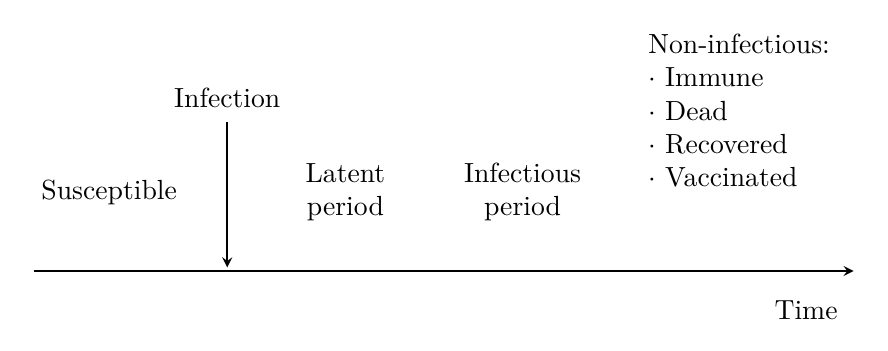
\begin{tikzpicture}[>= stealth, shorten >= 0pt,
                    auto, node distance=2.5cm, semithick]
\tikzstyle{every state}=[shape=rectangle, draw=none, 
                    semithick, inner sep=1pt, minimum size=0cm]
  \node[state] (start) at (0,0) {};
  \node[state] (end)   at (10.5,0) {};
  \node[state] (infection)       at (2.5,2.2) [inner sep=5pt] {Infection};
  \node[state] (infection_point) at (2.5,0) {};
  \node[state] (susceptible) at (1,1) {Susceptible};
  \node[state] (latent) at (4,1)
                            {\begin{tabular}{c}Latent\\period\end{tabular}};
  \node[state] (infectious) at (6.25,1)
                            {\begin{tabular}{c}Infectious\\period\end{tabular}};
  \node[state] (recovered) at(9, 2)
                            {\begin{tabular}{l}
                            Non-infectious:\\
                            $\cdot$ Immune\\ $\cdot$ Dead \\$\cdot$ Recovered \\$\cdot$ Vaccinated
                            \end{tabular}};
  \node[state] (Time) [below of=end, node distance=0.5cm, xshift=-0.65cm] {Time};
  \path[->]    (start) edge (end);
  \path[->]    (infection) edge (infection_point);
\end{tikzpicture}

\begin{center}
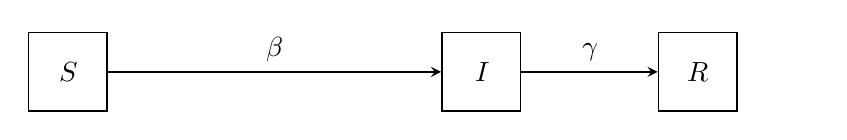
\begin{tikzpicture}[>= stealth, shorten >= 0pt,
                    auto, node distance=2.5cm, semithick]
\tikzstyle{every state}=[shape=rectangle, draw=black, 
                    semithick, inner sep=1pt, minimum size=1cm]
  \node[state] (S) at (1,0) {$S$};
  \node[state] (I) at (6.25,0) {$I$};
  \node[state] (R) at (9, 0) {$R$};
  \node[state] (end) at (10.5, 0) [draw=none, minimum size=0pt] {};
  \path[->]    (S) edge node {$\beta$} (I);
  \path[->]    (I) edge node {$\gamma$} (R);
\end{tikzpicture}
\end{center}
\end{frame}

\begin{frame}{Compartmental modeling: simple SIR case}
\protect\hypertarget{compartmental-modeling-simple-sir-case}{}
\begin{center}
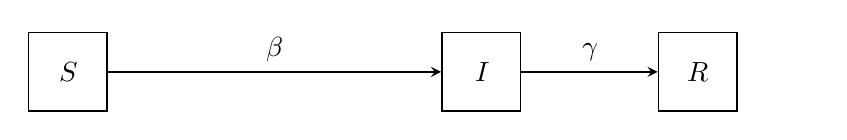
\begin{tikzpicture}[>= stealth, shorten >= 0pt,
                    auto, node distance=2.5cm, semithick]
\tikzstyle{every state}=[shape=rectangle, draw=black, 
                    semithick, inner sep=1pt, minimum size=1cm]
  \node[state] (S) at (1,0) {$S$};
  \node[state] (I) at (6.25,0) {$I$};
  \node[state] (R) at (9, 0) {$R$};
  \node[state] (end) at (10.5, 0) [draw=none, minimum size=0pt] {};
  \path[->]    (S) edge node {$\beta$} (I);
  \path[->]    (I) edge node {$\gamma$} (R);
\end{tikzpicture}
\end{center}

\[\left\{
\begin{aligned}
\frac{d}{dt} S & = - \frac{\beta}{N} I S \\
\frac{d}{dt} I & = \frac{\beta}{N} I S  -  \gamma I \\
\frac{d}{dt} R & = \gamma I
\end{aligned}
\right.\] \[S + I + R = N\]

See Harko, Lobo, and Mak (2014) for closed-form solutions.
\end{frame}

\begin{frame}{Compartmental modeling: theory of Rella et al. (2021)}
\protect\hypertarget{compartmental-modeling-theory-of-rella_2021}{}
\begin{center}
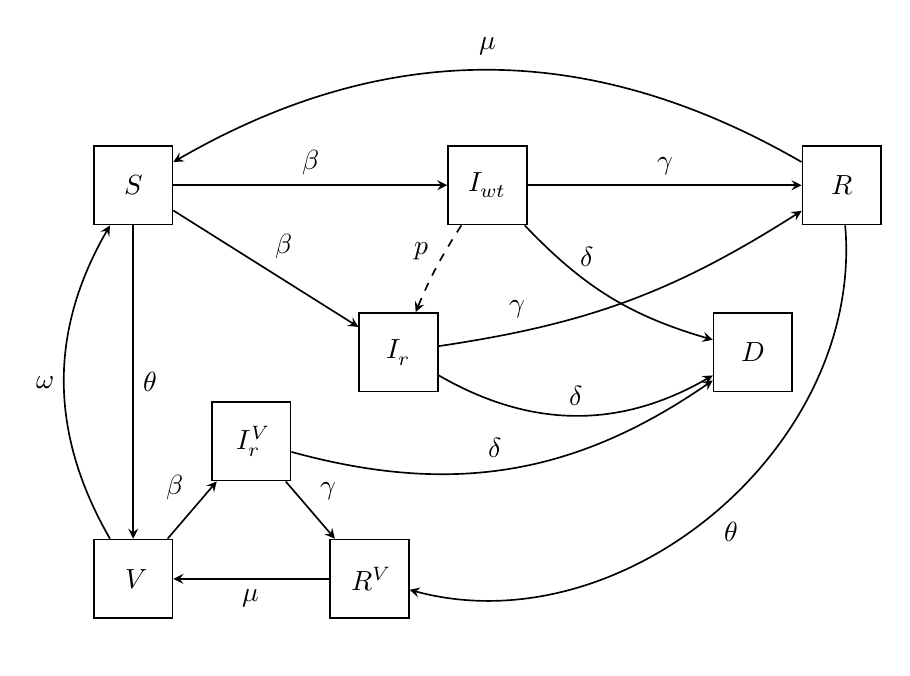
\begin{tikzpicture}[>= stealth, shorten >= 0pt,
                    auto, node distance=4.5cm, semithick]
\tikzstyle{every state}=[shape=rectangle, draw=black, 
                    semithick, inner sep=1pt, minimum size=1cm]
  \node[state] (S) {$S$};
  \node[state] (Iwt) [right of=S] {$I_{wt}$};
  \node[state] (R)   [right of=Iwt] {$R$};
  \node[state] (Ir)  [below right of=S, node distance=3cm, xshift=1.25cm] {$I_r$};
  \node[state] (D)   [right of=Ir] {$D$};
  \node[state] (V)   [below of=S, node distance=5cm] {$V$};
  \node[state] (IrV) [above right of=V, node distance=2.12cm, yshift=0.25cm] {$I_r^V$};
  \node[state] (RV)  [right of=V, node distance=3cm] {$R^V$};
  \path[->]    (S)   edge node {$\beta$} (Iwt);
  \path[->]    (S)   edge node {$\theta$} (V);
  \path[->]    (Iwt) edge node {$\gamma$} (R);
  \path[->]    (R)   edge [bend right=30] node [yshift=0.55cm] {$\mu$} (S);
  \path[->]    (Iwt) edge [bend right=15] node [yshift=0.25cm,xshift=-0.5cm] {$\delta$} (D);
  \path[->]    (R)   edge [bend left=55] node {$\theta$} (RV);
  \path[->]    (RV)  edge node {$\mu$} (V);
  \path[->]    (V)   edge node {$\beta$} (IrV);
  \path[->]    (IrV) edge node {$\gamma$} (RV);
  \path[->]    (IrV) edge [bend right=25] node {$\delta$} (D);
  \path[->]    (S)   edge node {$\beta$} (Ir);
  \path[->]    (Ir)  edge [bend right=12] node [yshift=-0.35cm, xshift=-1.2cm] {$\gamma$} (R);
  \path[->]    (Ir)  edge [bend right=30] node {$\delta$} (D);
  \path[->]    (Iwt) edge [style=dashed, bend right=5] node [yshift=0.45cm, xshift=-0.4cm] {$p$} (Ir);
  \path[->]    (V) edge [bend left=30] node {$\omega$} (S);
\end{tikzpicture}
\end{center}

\textbackslash end\{figure\}
\end{frame}

\begin{frame}{Modeling waves in epidemiologic trajectory}
\protect\hypertarget{modeling-waves-in-epidemiologic-trajectory}{}
\[\beta(t) = R_0(t) \times \gamma \times N^{-1}\] where
\[R_0(t) = \left\{\begin{aligned}
R_{0, \text{low}} 
\hspace{1em} \text{if}\hspace{1em}    & I > N \times p_h 
                            && \text{and} \hspace{1em} R_0(t - \Delta t) = R_{0, \text{high}} \\
R_{0, \text{high}}  
\hspace{1em} \text{if}\hspace{1em}    & I \times p_h \times p_l
                            && \text{and} \hspace{1em} R_0(t - \Delta t) = R_{0, \text{low}}
\end{aligned}\right.\] where \(I = I_{wt} + I_r + I_r^V\)
\end{frame}

\begin{frame}{Preliminary fit with time-invariant \(p_h\) and \(p_l\)}
\protect\hypertarget{preliminary-fit-with-time-invariant-p_h-and-p_l}{}
\includegraphics{interim_files/figure-beamer/unnamed-chunk-2-1.pdf}
\end{frame}

\begin{frame}{Preliminary fit with time-varying \(p_h\) and \(p_l\)}
\protect\hypertarget{preliminary-fit-with-time-varying-p_h-and-p_l}{}
\includegraphics{interim_files/figure-beamer/unnamed-chunk-4-1.pdf}
\end{frame}

\begin{frame}{Parameter specification (time-permitting)}
\protect\hypertarget{parameter-specification-time-permitting}{}
\begin{longtable}[]{@{}
  >{\raggedright\arraybackslash}p{(\columnwidth - 4\tabcolsep) * \real{0.1711}}
  >{\raggedright\arraybackslash}p{(\columnwidth - 4\tabcolsep) * \real{0.2368}}
  >{\raggedright\arraybackslash}p{(\columnwidth - 4\tabcolsep) * \real{0.5921}}@{}}
\toprule()
\begin{minipage}[b]{\linewidth}\raggedright
Parameter
\end{minipage} & \begin{minipage}[b]{\linewidth}\raggedright
Value
\end{minipage} & \begin{minipage}[b]{\linewidth}\raggedright
Interpretation
\end{minipage} \\
\midrule()
\endhead
\(\theta\) & 250.6335 & Vaccination rate (vaccines per day) \\
\(\delta\) & 7.3 \(\times\) 10,000 & Death rate (deaths per day) \\
\({R_0}_h\) & 2.2 & \(R_0\) during low caution \\
\({R_0}_l\) & 0.65 & \(R_0\) during high caution \\
\(\gamma\) & 1/14 & Inv. disease duration (days) \\
\(\mu\) & 1/(30 \(\times\) 12) & Inv. duration of natural immunity \\
\(\omega\) & 1/(30 \(\times\) 12) & Inv. duration of vaccine
protection \\
\bottomrule()
\end{longtable}
\end{frame}

\begin{frame}{Parameter specification (time-permitting)}
\protect\hypertarget{parameter-specification-time-permitting-1}{}
\begin{longtable}[]{@{}
  >{\raggedright\arraybackslash}p{(\columnwidth - 4\tabcolsep) * \real{0.1711}}
  >{\raggedright\arraybackslash}p{(\columnwidth - 4\tabcolsep) * \real{0.2368}}
  >{\raggedright\arraybackslash}p{(\columnwidth - 4\tabcolsep) * \real{0.5921}}@{}}
\toprule()
\begin{minipage}[b]{\linewidth}\raggedright
Parameter
\end{minipage} & \begin{minipage}[b]{\linewidth}\raggedright
Value
\end{minipage} & \begin{minipage}[b]{\linewidth}\raggedright
Interpretation
\end{minipage} \\
\midrule()
\endhead
\(p_{h,1}\) & 1/350 & Maximum prevalence before preventive measures in
1st wave \\
\(p_{h,2}\) & 1/63 & Maximum prevalence (2nd) \\
\(p_{h,3}\) & 1/165 & Maximum prevalence (3rd) \\
\(p_{h,4}\) & 1/325 & Maximum prevalence (4th) \\
\(p_{l,1}\) & 1/(350 \(\times\) 15) & Allowable prevalence before before
loosening measures (1st) \\
\(p_{l,2}\) & 1/(63 \(\times\) 15) & Allowable prevalence (2nd) \\
\(p_{l,3}\) & 1/(165 \(\times\) 2.5) & Allowable prevalence (3rd) \\
\(p_{l,4}\) & 1/(325 \(\times\) 17) & Allowable prevalence (4th) \\
\bottomrule()
\end{longtable}
\end{frame}

\begin{frame}{References}
\protect\hypertarget{references}{}
\hypertarget{refs}{}
\begin{CSLReferences}{1}{0}
\leavevmode\vadjust pre{\hypertarget{ref-CDC_2021}{}}%
CDC. 2021. {``First Confirmed Case of Omicron Variant Detected in the
United States.''} \emph{First Confirmed Case of Omicron Variant Detected
in the United States}.
\url{https://www.cdc.gov/media/releases/2021/s1201-omicron-variant.html}.

\leavevmode\vadjust pre{\hypertarget{ref-Harko_2014}{}}%
Harko, Tiberiu, Francisco SN Lobo, and MK3197716 Mak. 2014. {``Exact
Analytical Solutions of the Susceptible-Infected-Recovered (SIR)
Epidemic Model and of the SIR Model with Equal Death and Birth Rates.''}
\emph{Applied Mathematics and Computation} 236: 184--94.

\leavevmode\vadjust pre{\hypertarget{ref-Rella_2021}{}}%
Rella, Simon A, Yuliya A Kulikova, Emmanouil T Dermitzakis, and Fyodor A
Kondrashov. 2021. {``Rates of SARS-CoV-2 Transmission and Vaccination
Impact the Fate of Vaccine-Resistant Strains.''} \emph{Scientific
Reports} 11 (1): 15729.

\end{CSLReferences}
\end{frame}



\end{document}
